% Created 2024-06-16 Sun 00:13
% Intended LaTeX compiler: pdflatex
ocumentclass[10pt]{article}% =================================BASE====================================%
\documentclass[10pt]{report}
\usepackage[left=2cm,right=2cm,top=2cm,bottom=2cm]{geometry} % Marges
\usepackage[T1]{fontenc} % Nécessaire avec FrenchBabel
\usepackage[utf8]{inputenc} % Important pour symboles Francophones, é,à,etc
\usepackage{csquotes} % Recommandé par PDFLatex lors de la compilation. 


% Calligraphie
%\usepackage{lmodern} % Ça, ça set latin modern
%\usepackage{mathrsfs} %Permet la command \mathscr (Lettres attachées genre) \mathscr(B)

% Calligraphie
%\usepackage{pxfonts} % Met le texte ET les maths en Palatino + donne accès à des symboles math
\usepackage{palatino} % Cette commande met seulement le texte en police palatino
\usepackage{lmodern} % Pour les maths?
% Use lmodern for sans-serif
\usepackage{mathrsfs} % Permet la command \mathscr (Lettres attachées genre) \mathscr(B)





% Bibliographie
%\usepackage[backend=bibtex,style=phys,sorting=ynt]{biblatex}
\usepackage[backend=biber,sorting=ynt,style=ieee]{biblatex}
\addbibresource{/home/charlesedouard/Desktop/Travail/Documentation/master-bibliography.bib}



\usepackage{amsmath, amssymb, amsthm} % Symb. math. (Mathmode+Textmode) + Beaux théorèmes.
\usepackage{mathtools,cancel,xfrac} % Utilisation de boîtes \boxed{} + \cancelto{}{}, xfrac
\usepackage{graphicx, wrapfig} % Géstion des figures.
\usepackage{hyperref} % Permettre l'utilisation d'hyperliens.
\usepackage{color} % Permettre l'utilisation des couleurs.
\usepackage{colortbl} % Color tables
\usepackage[dvipsnames]{xcolor} % Couleurs avancées.
\usepackage{titling} % Donne accès à \theauthor, \thetitle, \thedate

% Physique
\usepackage{physics} % Meilleur package pour physicien. 


% Style
\usepackage{lipsum} % For fun
\usepackage{tikz} % Realisation de figures TIKZ.
\usepackage{empheq} % Boite autour de MULTIPLE équations
\usepackage{bbding}

% Français
\usepackage[french]{babel} % Environnements en Français.
% ==============================BASE-(END)=================================%



% ================================SETTINGS=================================%
% Pas d'indentation en début de paragraphe :
\setlength\parindent{0pt}
\setlength{\parskip}{0.15cm}

% Tableaux/tabular
% Espace vertical dans les tabular/tableaux
\renewcommand{\arraystretch}{1.2}
% Couleur des tableaux/tabular
\rowcolors{2}{violet!5}{}

% Couleurs de hyperliens :
\definecolor{mypink}{RGB}{147, 0, 255}
\hypersetup{colorlinks, 
             filecolor=mypink,
             urlcolor=mypink, 
             citecolor=mypink, 
             linkcolor=mypink, 
             anchorcolor=mypink}


\usepackage{titling} % Donne accès à \theauthor, \thetitle, \thedate

% Physique
\usepackage{physics} % Meilleur package pour physicien. 


% Style
\usepackage{lipsum} % For fun
\usepackage{tikz} % Realisation de figures TIKZ.
\usepackage{empheq} % Boite autour de MULTIPLE équations

% Français
\usepackage[french]{babel} % Environnements en Français.
% ==============================BASE-(END)=================================%





% ================================SETTINGS=================================%
% Pas d'indentation en début de paragraphe :
\setlength\parindent{0pt}
\setlength{\parskip}{0.15cm}

% Tableaux/tabular
% Espace vertical dans les tabular/tableaux
\renewcommand{\arraystretch}{1.2}
% Couleur des tableaux/tabular
\rowcolors{2}{violet!5}{}

% Couleurs de hyperliens :
\definecolor{mypink}{RGB}{147, 0, 255}
\hypersetup{colorlinks, 
             filecolor=mypink,
             urlcolor=mypink, 
             citecolor=mypink, 
             linkcolor=mypink, 
             anchorcolor=mypink}


% Numéros d'équations suivent les sections :
\numberwithin{equation}{section} 

% Les « captions » sont en italique et largeur limitée
\usepackage[textfont = it]{caption} 
\captionsetup[wrapfigure]{margin=0.5cm}

% Retirer l'écriture en gras dans la table des matières
\usepackage{tocloft}
\renewcommand{\cftsecfont}{\normalfont}
\renewcommand{\cftsecpagefont}{\normalfont}

% Change bullet style
\usepackage{pifont}
\usepackage{enumitem}
%\setlist[itemize,1]{label=\ding{224}}
\setlist[itemize,1]{label=\ding{239}}
\renewcommand{\boxtimes}{\blacksquare}
% ================================SETTINGS=================================%



% ==============================NEWCOMMANDS================================%

% Vecteurs de base :
\newcommand{\nvf}{\vb{\hat{n}}}
\newcommand{\ivf}{\vb{\hat{i}}}
\newcommand{\jvf}{\vb{\hat{j}}}
\newcommand{\kvf}{\vb{\hat{k}}}
\newcommand{\uu}{\vb{u}}
\newcommand{\vv}{\vb{v}}
\newcommand{\ust}{\vb{u}_{\ast}}

% Physics empty spaces 
\newcommand{\typical}{\vphantom{A}}
\newcommand{\tall}{\vphantom{A^{x^x}_p}}
\newcommand{\grande}{\vphantom{\frac{1}{xx}}}
\newcommand{\venti}{\vphantom{\sum_x^x}}
\newcommand{\pt}{\hspace{1pt}} % One horizontal pt space

% Moyenne numérique entre deux points de grilles. 
\newcommand{\xmean}[1]{\overline{#1}^x}
\newcommand{\ymean}[1]{\overline{#1}^y}
\newcommand{\zmean}[1]{\overline{#1}^z}
\newcommand{\xymean}[1]{\overline{#1}^{xy}}

% Tilde over psi
\newcommand{\tpsi}{\tilde{\psi}}
\newcommand{\tphi}{\tilde{\phi}}

% Nota Bene env : (\ding{89})
%\newcommand{\nb}{$\boxed{\text{\footnotesize\EightStarConvex}\pt \mathfrak{N. B.}}$\hspace{4pt}}
\newcommand{\nb}{\underline{{\footnotesize\EightStarConvex}\pt $\mathfrak{N.B.}$\vphantom{p}}\hspace{3pt}}


% Define the nota bene environment
\usepackage{tcolorbox}
\newtcolorbox{notabene}{
     colback=blue!5,
     colframe=black,
     boxrule=0.5pt,
     arc=2pt,
     left=5pt,
     right=5pt,
     top=5pt,
     bottom=5pt,
}


\newcommand{\cmark}{\ding{52}}
\newcommand{\xmark}{\ding{55}}
% ==============================NEWCOMMANDS================================%



% ==============================PAGE-TITRE=================================%
% Titlepage 
\newcommand{\mytitlepage}{
\begin{titlepage}
\begin{center}
{\Huge Contrat Été 2023 \par}
\vspace{2cm}
{\Huge \MakeUppercase{\thetitle} \par}
\vspace{2cm}
RÉALISÉ DANS LE CADRE\\ D'UN PROJET POUR \par
\vspace{2cm}
{\Huge ISMER--UQAR \par}
\vspace{2cm}
{\thedate}
\end{center}
\vfill
Rédaction \\
{\theauthor}\\
\url{charles-edouard.lizotte@uqar.ca}\\
ISMER-UQAR\\
Police d'écriture : \textbf{CMU Serif Roman}
\end{titlepage}
}
% ==============================PAGE-TITRE=================================%



% =================================ENTÊTE==================================%
\usepackage{fancyhdr}
\pagestyle{fancy}
\setlength{\headheight}{13pt}
\renewcommand{\headrulewidth}{0.025pt} % Ligne horizontale en haut

\fancyhead[R]{\textit{\thetitle}}
\fancyhead[L]{\ \thepage}
\fancyfoot[R]{\textit{\theauthor}}
\fancyfoot[L]{}
\fancyfoot[C]{} 
% =================================ENTÊTE==================================%
\author{Charles-Édouard Lizotte}
\date{16/06/2023}
\title{Carnet de bord, Université McGill}
\hypersetup{
 pdfauthor={Charles-Édouard Lizotte},
 pdftitle={Carnet de bord, Université McGill},
 pdfkeywords={},
 pdfsubject={},
 pdfcreator={Emacs 27.1 (Org mode 9.6.7)}, 
 pdflang={French}}
\begin{document}

\mytitlepage
\tableofcontents\newpage



\section{Considérations en lien avec le premier pas de temps}
\label{sec:org085b989}
\subsection{Mise en contexte}
\label{sec:orgca33a7b}
\begin{wrapfigure}{r}{0.5\textwidth} \vspace{-\baselineskip} \centering
\centering
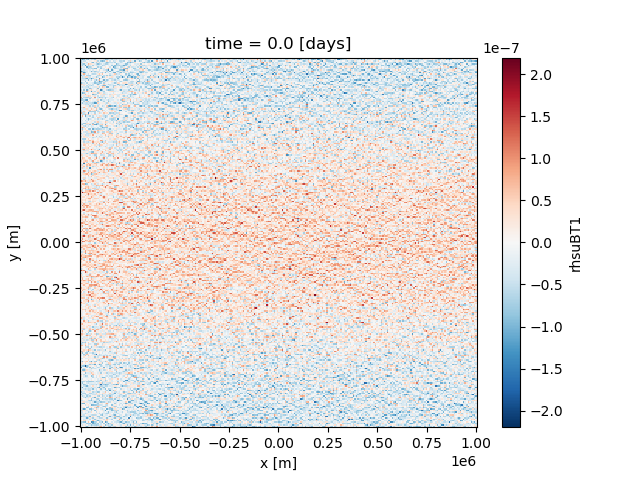
\includegraphics[width=0.48\textwidth]{figures/debuggage/2023_06_12_RHSuBTmudpack.png}
\caption{\label{fig:org690b49c}Premier "RHS" barotrope réalisé à l'aide du module MUDPACK. Par "RHS" barotrope, on considère la variation en y de \(\psi_{BT}\), soit \(\delta \psi_{BT}\), donc \(\pdv*{(\delta \psi_{BT})}{y}\).}
\end{wrapfigure}


La semaine passée (voir \href{rapport-2023-06-03.org}{rapport précédent}), en réalisant des tests et en débuggant sur les premiers pas de temps du modèle en eau peu profonde, j'ai fait la découverte d'une erreur conceptuelle importante.
Les corrections barotropes (ou les \emph{RHS}) des deux modèles (\emph{FFTW} et \emph{MUDPACK}) n'avaient pas du tout le même signe.
Pour mettre en contexte, le premier pas de temps calcule le \emph{RHS} à partir d'un courant purement positif sur l'entièreté du domaine.
En effet, le premier champs vectoriel du courant (its=1) est issu d'un bruit aléatoire entre 0 et 0.01 \(ms^{-1}\).
Cette technique primitive permet d'introduire de légères perturbations qui -- bien que non-essentielles à la production baroclinique -- aide le modèle à en créer plus rapidement.
Sans cette méthode, on fait plutôt condiance aux perturbations induites par le bruits numérique pour créer de l'instabilité barocline, ce qui peut prendre beaucoup de temps selon David et Louis-Philippe. \bigskip

Comme ce premier champ est uniquement positif et que le vent est plutôt faible, les termes d'advections dominent , ce qui induit un \emph{RHS}, lui-aussi, entièrement positif.
Et comme le courant est entièrement nul dans les couches inférieures, le RHS est nul dans ces mêmes couches. \bigskip

\begin{wrapfigure}{l}{0.5\textwidth} \vspace{-\baselineskip} \centering
\centering
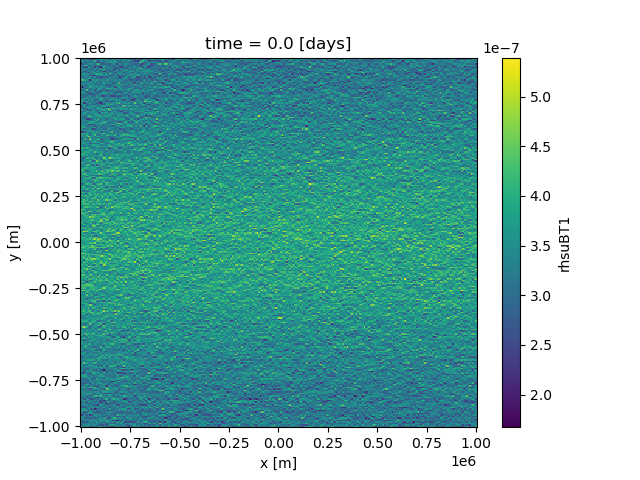
\includegraphics[width=0.48\textwidth]{figures/debuggage/2023_06_12_RHSuBTfftw.png}
\caption{\label{fig:orge6e4492}Partie barotrope du "RHS" du modèle "FFTW". On additionne ainsi la partie barotrope du "RHS" avec la correction de la pression due à la surface fixe.}
\end{wrapfigure}

\subsection{Courant moyen}
\label{sec:org71977d3}

Il est possible de décomposer ce RHS en quantités barotrope et baroclines.
Comme ce \emph{RHS} positif est assez uniforme, on doute qu'une partie devrait se retrouver dans le \emph{RHS} barotrope.
Dès lors, on voit que le modèle \emph{shallow water FFT} produit un \emph{RHS} uniquement positif (figure \ref{fig:orge6e4492}), tandis que le modèle \emph{MUDPACK} produit des quantités mixtes (voir figure \ref{fig:org690b49c}).
La correction positive sur tout le domain est donc abscente de la solution proposée par MUDPACK.
Mais pourquoi est-ce le cas?\bigskip

Mathématiquement, imaginons un courant moyen induit sur tout le domaine \(\overline{\uu}\), ce courant satisferait les conditions frontières, ce qui en fait une solution valide.
Par contre, comme ce dernier est définit par
\begin{equation}
   \uu = \overline{\uu} + \uu' = - \curl(\psi\kvf),
\end{equation}
il faudrait impérativement que la fonction de courant (\(\psi\)) satisfasse la relation
\begin{equation}
\label{eq:orge088110}
   \psi = f(x,y) - \overline{\uu} y.
\end{equation}

Où \(f(x,y)\) est une solution périodique quelconque. 
Malheureusement, la solution \ref{eq:orge088110} ne peut possiblement pas satisfaire la continuité aux frontières d'un domaine périodique, car \(\psi(y) = \overline{\uu} y\) n'est pas du tout une fonction périodique.
Il faut donc en déduire que la fonction de courant \(\psi\) ne contient pas toute l'information nécessaire à la solution.\bigskip

\textbf{N.B.\ } \begin{minipage}[t]{0.94\linewidth}
   \itshape Mentionnons que l'existence de la solution \ref{eq:orge088110} est seulement possible dans une domaine doublement périodique.
   Dans un domaine fermée, la conservation de la masse empêche ce genre de solution d'exister. Bref, en moyenne \(\overline{\uu_i h_i} = 0\).
\end{minipage}


\section{Argument mathématique vis-à-vis la méthode}
\label{sec:orgfe2ffd7}

\subsection{Mise en contexte}
\label{sec:org1bffeae}
Concrétement, la méthode courante consiste à prendre l'équation
\begin{equation}
   \laplacian{\psi^{t+\delta t}} = \kvf\cdot\curl{\uu^{t+\delta t}}.
\end{equation}
et de la décomposer en ses partie importantes à l'aide de la méthode des différences finies.
Soit
\begin{equation}
   \laplacian(\psi^t + \Delta t\cdot\delta \psi) = \kvf\cdot\curl(\uu^t + \Delta t\cdot\vec{RHS}^t - \Delta t\cdot\gradient{\phi}).
\end{equation}
Comme \(\laplacian{\psi^t} = \kvf\cdot\curl{\uu^t}\), on pouvait affirmer que
\begin{equation}
\label{eq:org8bce997}
   \laplacian(\delta \psi_{BT} + \delta \psi_{BC}) = \kvf\cdot\curl(\vec{RHS}^t_{BT} + \vec{RHS}^t_{BC} - \gradient{\phi}),
\end{equation}
et qu'on pouvait diviser le RHS en partie barotrope et barocline.
Ici, on faisait l'assomption que cette équation était séparable en deux sections, de sorte à obtenir une équation seulement pour la partie barocline,
\begin{equation}
\label{eq:org83c7440}
   \laplacian(\delta \psi_{BT}) = \kvf\cdot\curl(\vec{RHS}^t_{BT} - \cancelto{0}{\gradient{\phi}}).
\end{equation}
Une fois ici, on solvait l'équation
\begin{equation}
   \laplacian(\delta \psi_{BT}) = \kvf\cdot\qty(\curl{\vec{RHS}^t_{BT}})
\end{equation}
et l'on retrouvait
\begin{equation}
   \qty(\pdv{\uu}{t})^t = \vec{RHS}^t_{BC} + \kvf\times\gradient(\delta\psi_{BT}).
\end{equation}
Bref, il existe une erreur conceptuelle du passage de \ref{eq:org8bce997} à \ref{eq:org83c7440} et je tenterai de le démontrer dans la section suivante.


\subsection{Considérations sur la fonction de courant barotrope}
\label{sec:org03811da}
Après y avoir pensé très fort, on peut affirmer que
\begin{equation}
   \laplacian{\psi_{BT}} \not= \kvf\cdot\qty(\curl{\uu_{BT}}).
\end{equation}

Cette inégalité est reliée à la manière qu'on définit \(\uu_{BT}\).
Pour mettre ceci en évidence, rappellons que pour chaque fonction de courant \(\psi_i\) de notre modèle
\begin{equation}
   \laplacian{\psi_i} = \kvf\cdot\qty(\curl{\uu_i}).
\end{equation}

On peut donc sommer l'ensemble de ces équations et l'on obtient
\begin{equation}
   \sum_i^Nh_i\pt\laplacian{\psi_i} = \kvf\cdot \sum_i^N h_i\pt \qty(\curl{\uu_i}).
\end{equation}

Avec quelques règles de dérivation et des identités, on parvient à une forme générale d'où émergent les quantités barotropes
\begin{align}
   \sum_i^N \bigg[ \underbrace{\grande\laplacian(h_i\psi_i)}_{\laplacian{\psi_{BT}}} - \psi_i\pt\qty(\laplacian{h_i}) - 2 \laplacian{h_i}\laplacian{\psi_i}\bigg]
    = \kvf\cdot \sum_i^N \bigg[ \underbrace{\grande\curl(h_i \uu_i)}_{\curl{\uu_{BT}}}  - \qty(\gradient{h_i})\times\uu_i\bigg],
\end{align}
qu'on simplifie en divisant par \(H\) pour parvenir à
\begin{align}
\label{eq:orgf400762}
   &\laplacian{\psi_{BT}} - \sum_i^N \bigg[ \frac{\psi_i}{H} \qty(\laplacian{h_i}) + \frac{2}{H} \laplacian{h_i}\laplacian{\psi_i}\bigg]
    = \kvf\cdot  \qty(\curl{ \uu_{BT}}) - \kvf\cdot \qty[\sum_i^N \frac{1}{H} \qty(\gradient{h_i})\times\uu_i],\nonumber\\
%
   &\laplacian{\psi_{BT}}
    = \kvf\cdot  \qty(\curl{ \uu_{BT}}) + \underbrace{\qty[ \frac{\psi_i}{H} \qty(\laplacian{h_i}) + \frac{2}{H} \laplacian{h_i}\laplacian{\psi_i}  -
\sum_i^N \frac{\kvf}{H}\cdot\qty(\gradient{h_i}\times\uu_i)]}_\text{Résidu}.
\end{align}

Donc, si l'on définit la correction barotrope comme une moyenne, on doit se résoudre à ce que
\begin{equation}
\label{eq:org6784102}
   \boxed{\hspace{0.3cm}\laplacian{\psi_{BT}} \not= \kvf\cdot  \qty(\curl{ \uu_{BT}}).\hspace{0.3cm}}
\end{equation}

\nb\begin{minipage}[t]{0.9\linewidth}
\itshape Par contre, il est possible que tous les termes à droite de l'équation \ref{eq:orgf400762} s'annulent.
Si c'est le cas nous pouvons conserver la formulation originale, mais je ne serai malheureusement pas celui qui va le vérifier.
Intuitivement, je ne vois pas pourquoi ces termes s'annuleraient.
David a mentionné qu'il est possible que l'inégalité \ref{eq:org6784102} soit fausse et que ça viendrait seulement de la manière éronnée que nous définissons notre courant barotrope.
Dans la section suivante, nous tentons une solution en lien avec la première section et cette dernière inégalité.
\end{minipage}

\subsection{Considérations sur la fonction de courant barotrope (retour sur le chapitre 5.3)}
\label{sec:orgcdf3ae7}
L'équation
\begin{equation}
   \laplacian{\psi_i} = \kvf\cdot\curl{\uu_i},
\end{equation}
décrit ce qu'on appelle la \textbf{balance géostrophique} et elle relie essentiellement la vorticité potentielle et la fonction de courant géostrophique.
Comme nous somme en \emph{shallow water Quasi-Geostrophic}, cette équation tient la route.
Essentiellement, on peut définir une fonction de courant géostrophique (p.177), car au premier ordre
\begin{equation}
   \divergence{\uu_0} = 0.
\end{equation}
Cette notion, vient principalement du fait qu'on peut relier \(\psi\) avec \(\eta\), mais qu'on peut aussi relier \(\eta\) avec \(\zeta\).
Donc ça vient de la balance géostrophique et ça apparait à l'équation (5.63 [p.181, Vallis]), car
\begin{align}
&&f_0 u_0 = -\pdv{\eta_0}{y},
&& f_0 v_0 = \pdv{\eta_0}{x} &&
\end{align}



\section{Solution}
\label{sec:orge3265b8}
\begin{wrapfigure}[18]{r}{0.5\textwidth} \vspace{-\baselineskip} \centering
\centering
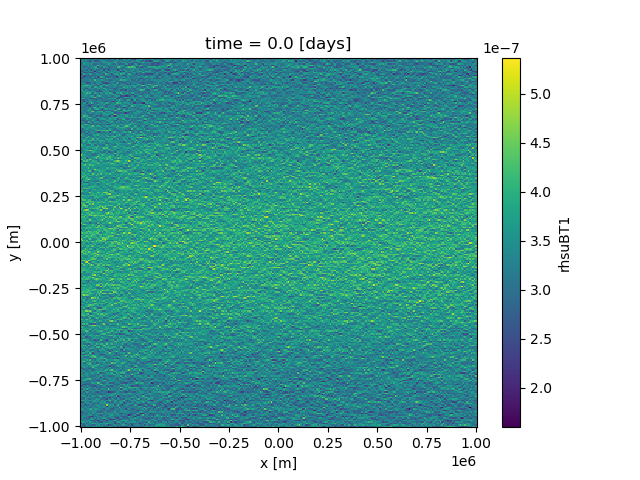
\includegraphics[width=0.48\textwidth]{figures/debuggage/2023_06_14_RHSuBTmudpack.png}
\caption{\label{fig:orgc5616e0}Nouvelle partie barotrope entière du RHS au premier pas de temps. On compte ici la moyenne barotrope du "RHS", ainsi que la correction appliquée par la fonction de courant.}
\end{wrapfigure}

La relation entre la variation de \(\psi\) et celle du rotationnel de notre \emph{RHS}, soit
\begin{equation}
   \laplacian(\delta \psi) = \kvf\cdot\curl(\vec{RHS}^t - \gradient{\phi}),
\end{equation}
tient toujours la route et on pourrait l'utiliser à notre avantage.\bigskip

Comme nous l'avons vu dans la section 1, on définit la correction barotrope à l'aide de l'équation \(\psi_{BT} \propto \kvf\cdot\curl(\uu_{BT})\), ce qui fait disparaître tout courant barotrope moyenné sur le domaine.
Essentiellement, cette différence créait un écart dignificatif entre les \emph{RHS} des modèles solutionnés par \emph{FFTW} et \emph{MUDPACK}.
Ensuite, nous avons vu que, mathématiquement, il y a un problème.\bigskip

La solution est de calculer le \emph{RHS} barotrope à l'aide de
\begin{equation}
   \vec{RHS}^t_{BT} = \kvf\cdot \sum_i^N \bigg[ \underbrace{\grande\curl(h^t_i \uu^t_i)}_{\curl{\uu^t_{BT}}}  - \qty(\gradient{h^t_i})\times\uu^t_i\bigg].
\end{equation}

Ensuite on conserve la moyenne barotrope du \emph{RHS} en banque, soit
\begin{equation}
   \xymean{RHS^t_{BT}} = \qty(\frac{1}{nx\cdot ny})\sum_{i,j}^{nx,ny} \vec{RHS}^t_{BT}[i,j].
\end{equation}
Et l'on additionne les trois partie pour avoir la solution finale
\begin{equation}
   \vec{RHS}^t = \underbrace{\venti\xymean{RHS^t_{BT}} \ + \ \delta \psi_{BT}}_\text{Partie barotrope}\ + \ \underbrace{\venti\vec{RHS}^t_{BC}}_\text{Barocline}.
\end{equation}

Et il semble que ça fonctionne.
On peut maintenant comparter les figures \ref{fig:orge6e4492} et \ref{fig:orgc5616e0} et voir que les deux se ressemble beaucoup, pour ne pas dire qu'ils sont identiques. \bigskip

\nb\begin{minipage}[t]{0.9\linewidth}
\itshape Nous n'avions pas ce problème lorsque nous trouvions le gradient de pression de surface à l'aide des transformées de Fourier, car on calculait un par de temps intermédiaire et ensuite on corrigeait le prochain pas de temps. Maintenant, on efface carrément le RHS pour retrouver un RHS avec MUDPACK. C'est donc un nouveau problème.
\end{minipage}


\section{{\bfseries\sffamily DONE} Résultats et comparaison des deux solveurs}
\label{sec:orgfdc1f4a}
Dans cette sections, nous comparons les résultats obtenus avec les deux modèles, soit celui donc le gradient de pression de surface est solvé à l'aide de transformée de Fourrier et celui donc la correction de la fonction de courant barotrope est solvée par technique \emph{multigrid} (MUDPACK).\bigskip

\nb\begin{minipage}[t]{0.9\linewidth}
\itshape 
eta1 ne dénote par la même quantité dans les deux cas.
Pour le modèle FFTW, eta1 dénote la pression de surface.
Tandis que la même quantité dénote la correction de la fonction de courant dans le modèle solvé à l'aide de MUDPACK.   
\end{minipage}
\newpage

\subsection{Spin up}
\label{sec:org3e7d364}
Les deux modèles accumulent de l'énergie.
Du côté de \emph{MUDPACK}, on observe l'appararition de lignes horizontales dans le rotationnel de la première couche, ainsi qu'un genre de \emph{bruit} numérique dans la divergence (Voir figures \ref{tab:org7584bb2} et \ref{tab:org1045079}).
On ne voyait pas ça dans le cas FFT (Voir figures \ref{tab:org7584bb2} et \ref{tab:org1045079})


\begin{table}[!htpb]
\caption{\label{tab:org7584bb2}Diagrammes de Hovmoller entre 0 et 250 jours. Pression de surface calculée à l'aide de FFTW à gauche. Correction psi barotrope à l'aide de MUDPACK à droite.}
\centering
\begin{tabular}{ll}
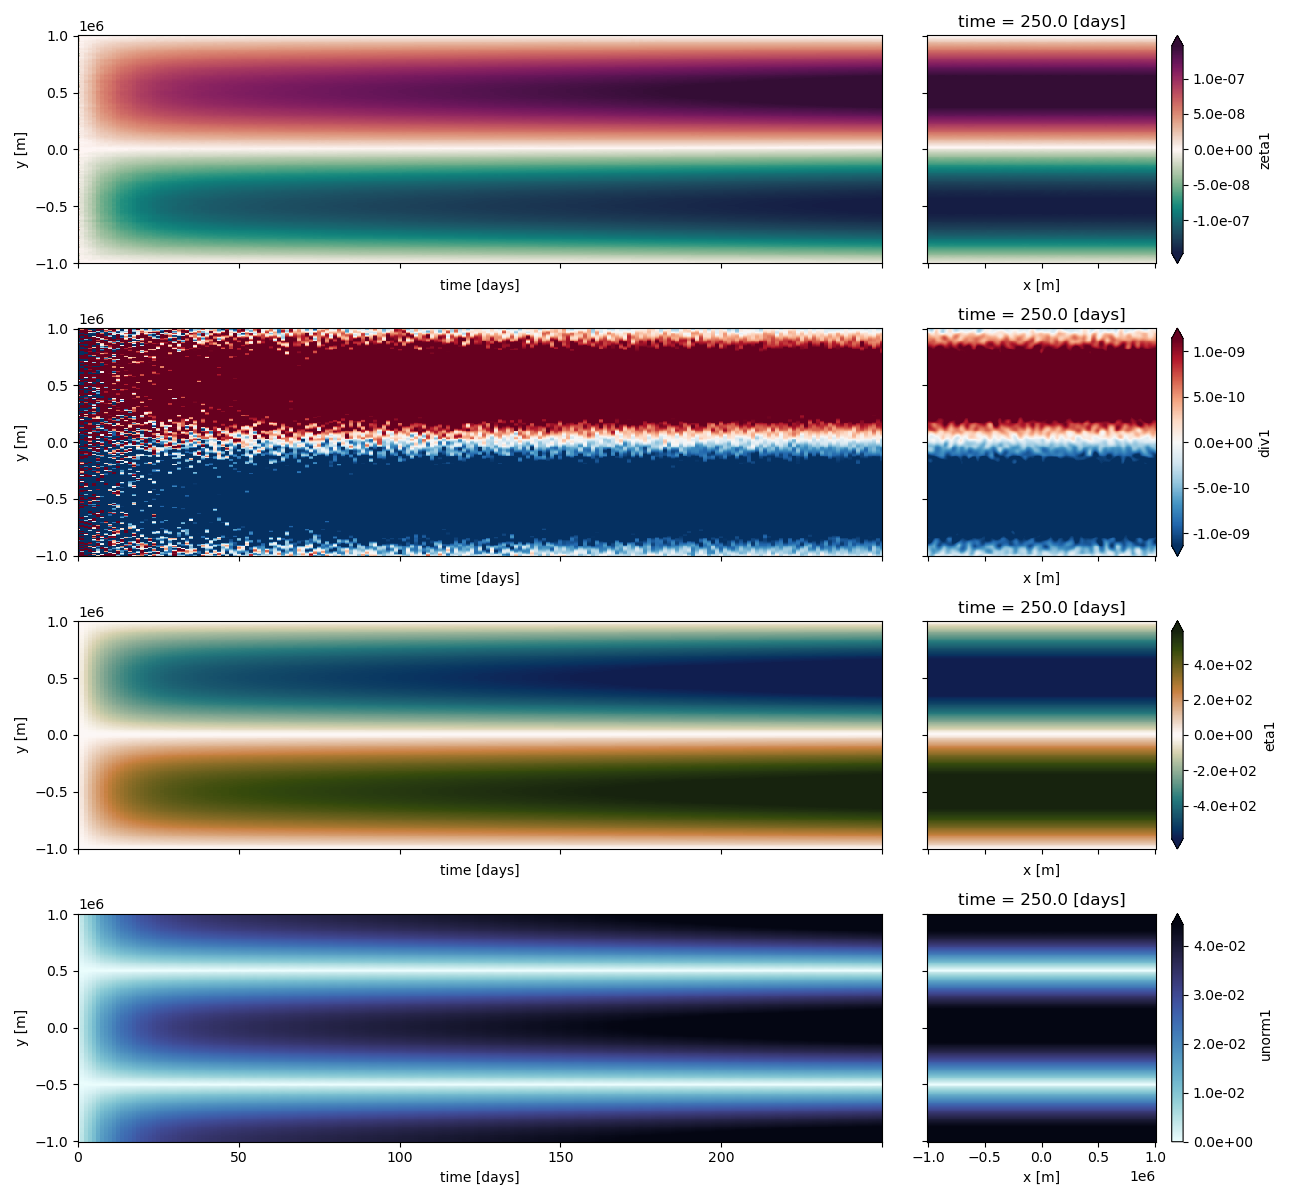
\includegraphics[width=0.5\textwidth]{figures/tests/2023-06-15_hovmoller1_t=250days_fft.png} & 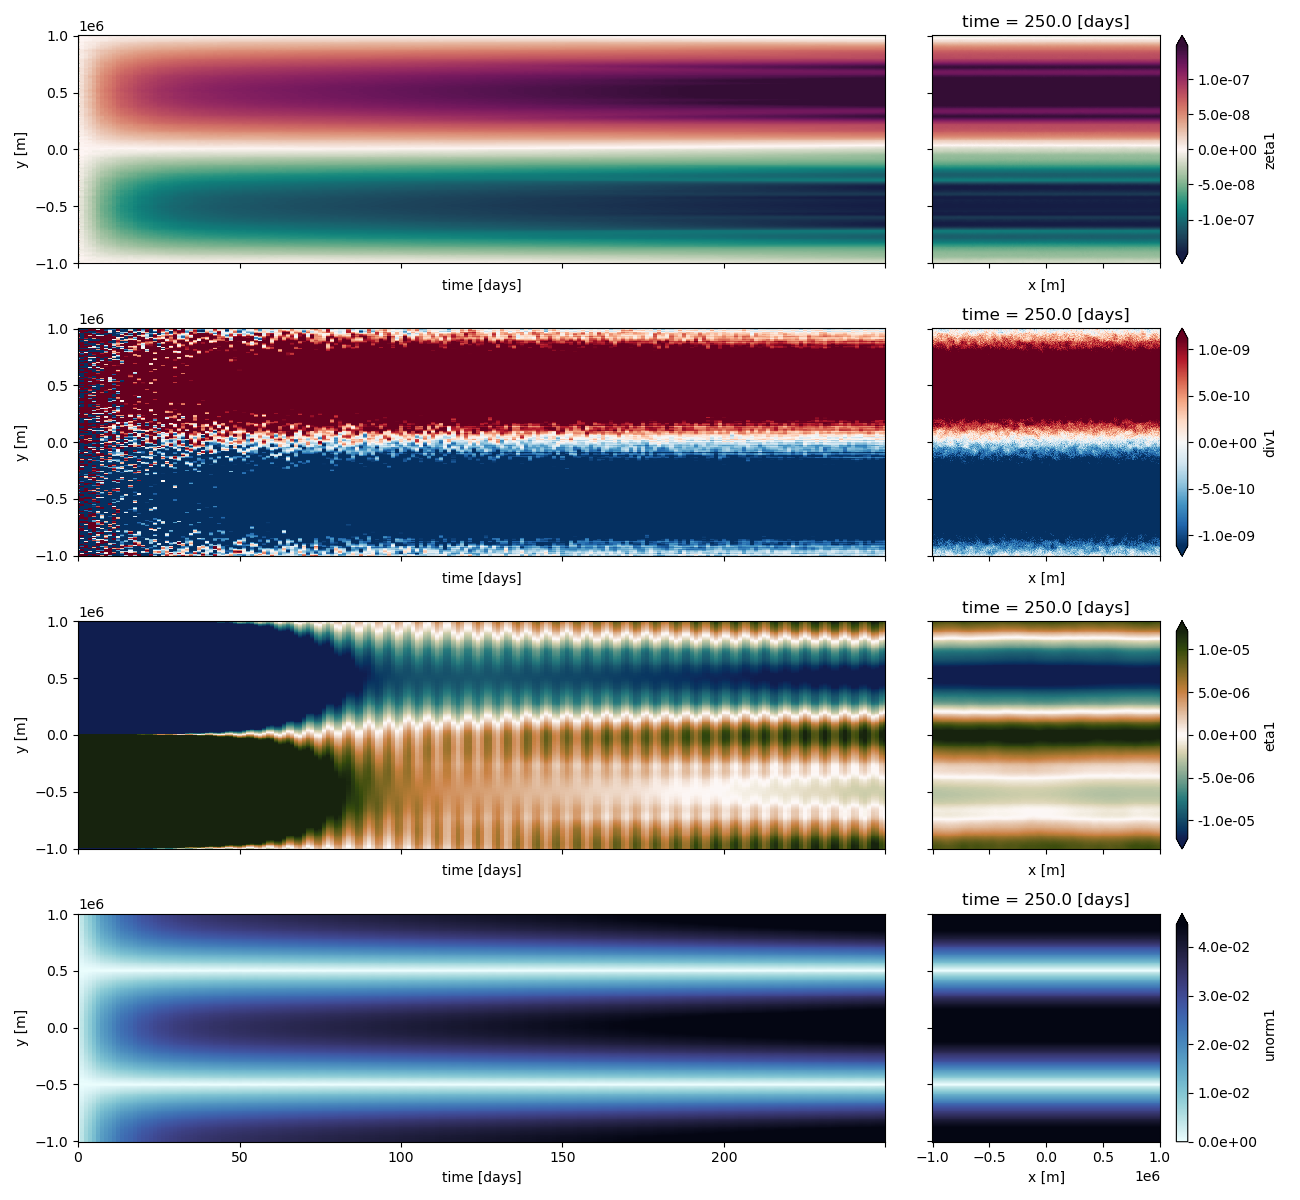
\includegraphics[width=0.5\textwidth]{figures/tests/2023-06-16_hovmoller1_t=250days_mud.png}\\[0pt]
\end{tabular}
\end{table}
\newpage

\subsection{Phase de production des instabilités baroclines}
\label{sec:org9feaf54}
Le cisaillement des vitesses induit la production d'instabilités baroclines.
Malgré de légères différences pendant le \emph{spin up}, la phase de production barocline se passe plutôt au même moment que dans l'autre modèlem, ce qui est encourageant.

\begin{table}[htbp]
\caption{\label{tab:org1045079}Diagrammes de Hovmoller entre 0 et 1000/950 jours. Pression de surface calculée à l'aide de FFTW. Correction psi barotrope à l'aide de MUDPACK à droite.}
\centering
\begin{tabular}{ll}
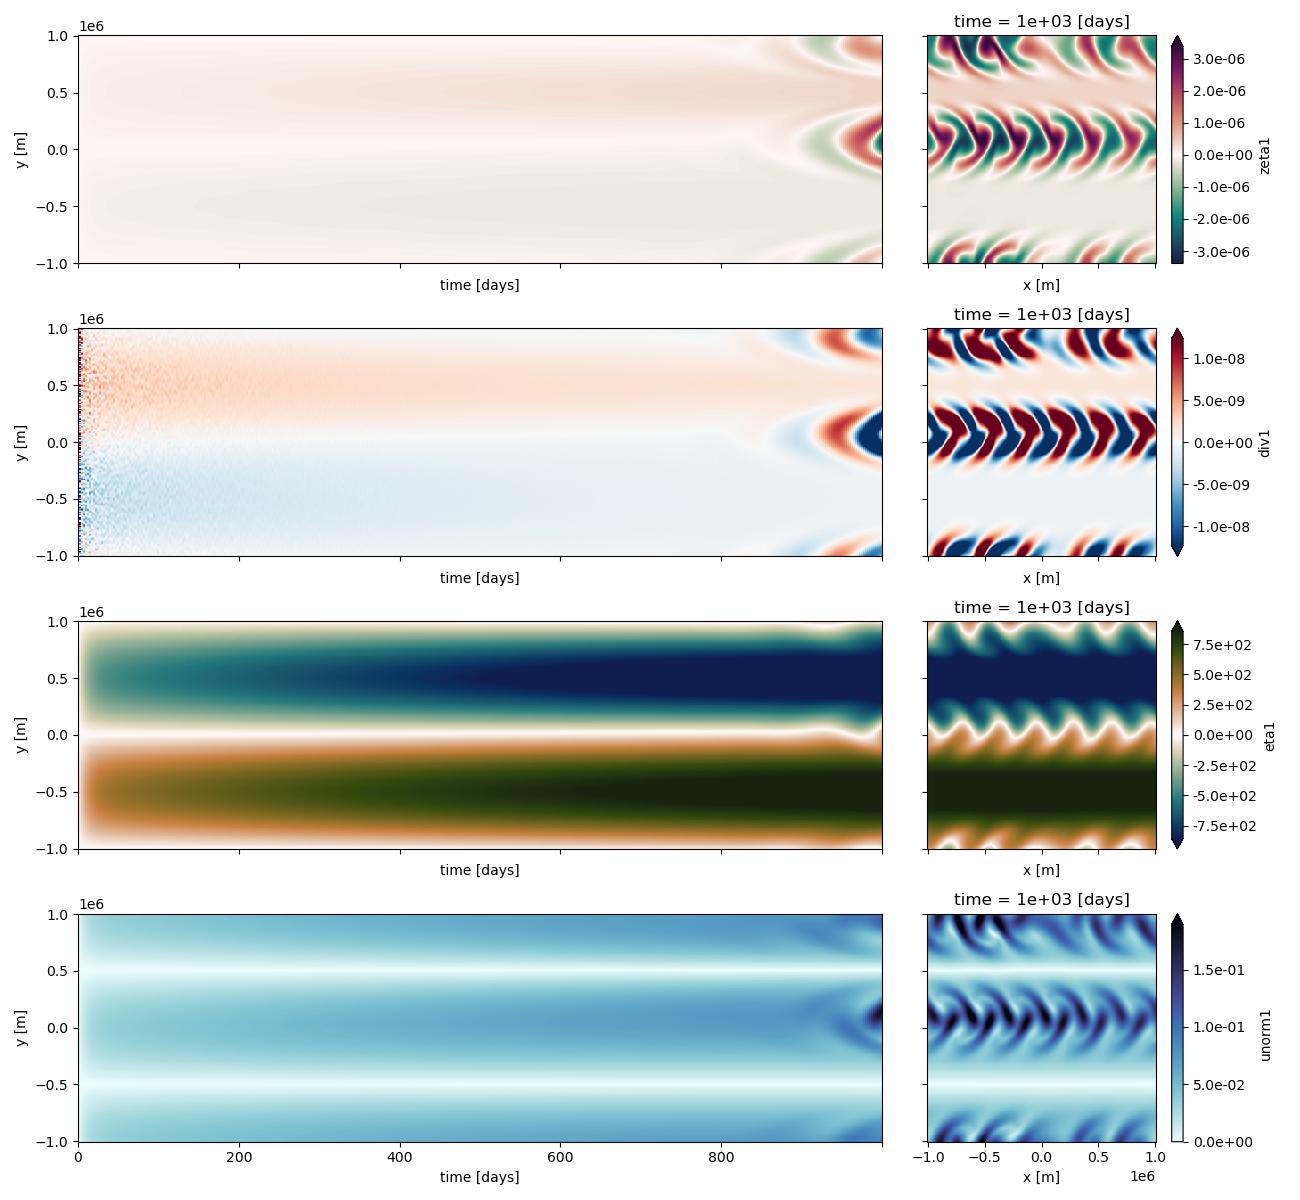
\includegraphics[width=0.5\textwidth]{figures/tests/2023-06-15_hovmoller1_t=1000days_fft.png} & 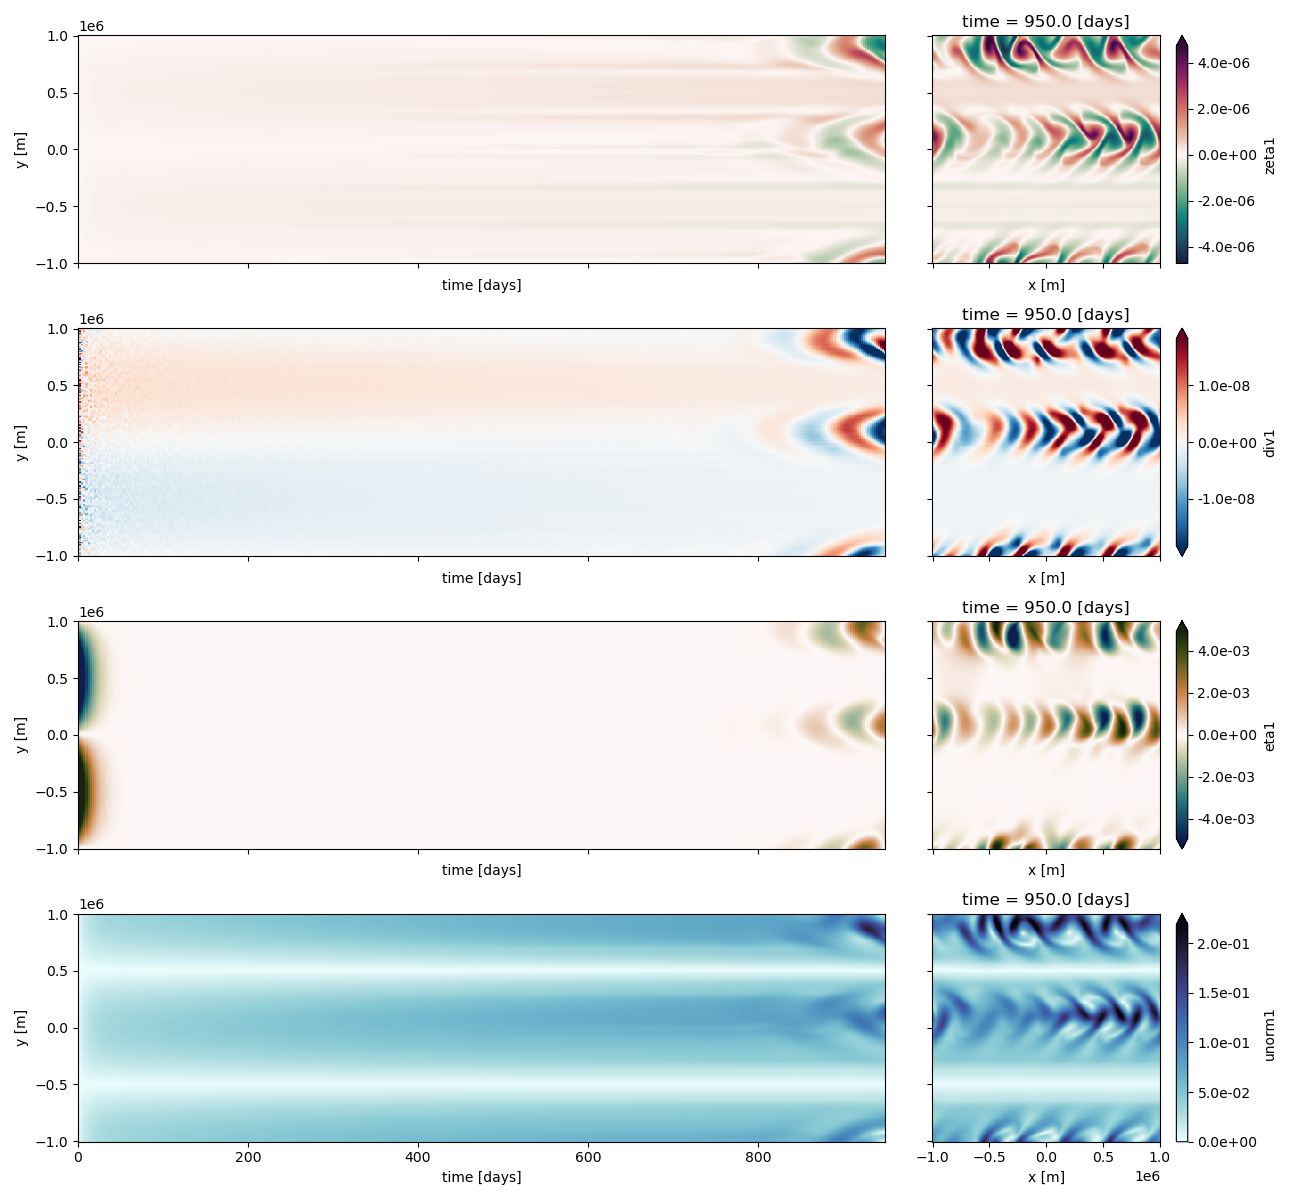
\includegraphics[width=0.5\textwidth]{figures/tests/2023-06-16_hovmoller1_t=950days_mud.png}\\[0pt]
\end{tabular}
\end{table}
\newpage

\subsection{Stabilité barocline}
\label{sec:orgcfe80f7}
Les tourbillons remplissent le domaine.
Une fois la phase de production baroclinique terminée, on ne voit que très peu de différence entre les deux modèles numériques.

\begin{table}[htbp]
\caption{\label{tab:org426c4f5}Diagrammes de Hovmoller entre 0 et 1500 jours. Pression de surface calculée à l'aide de FFTW. Correction psi barotrope à l'aide de MUDPACK à droite.}
\centering
\begin{tabular}{ll}
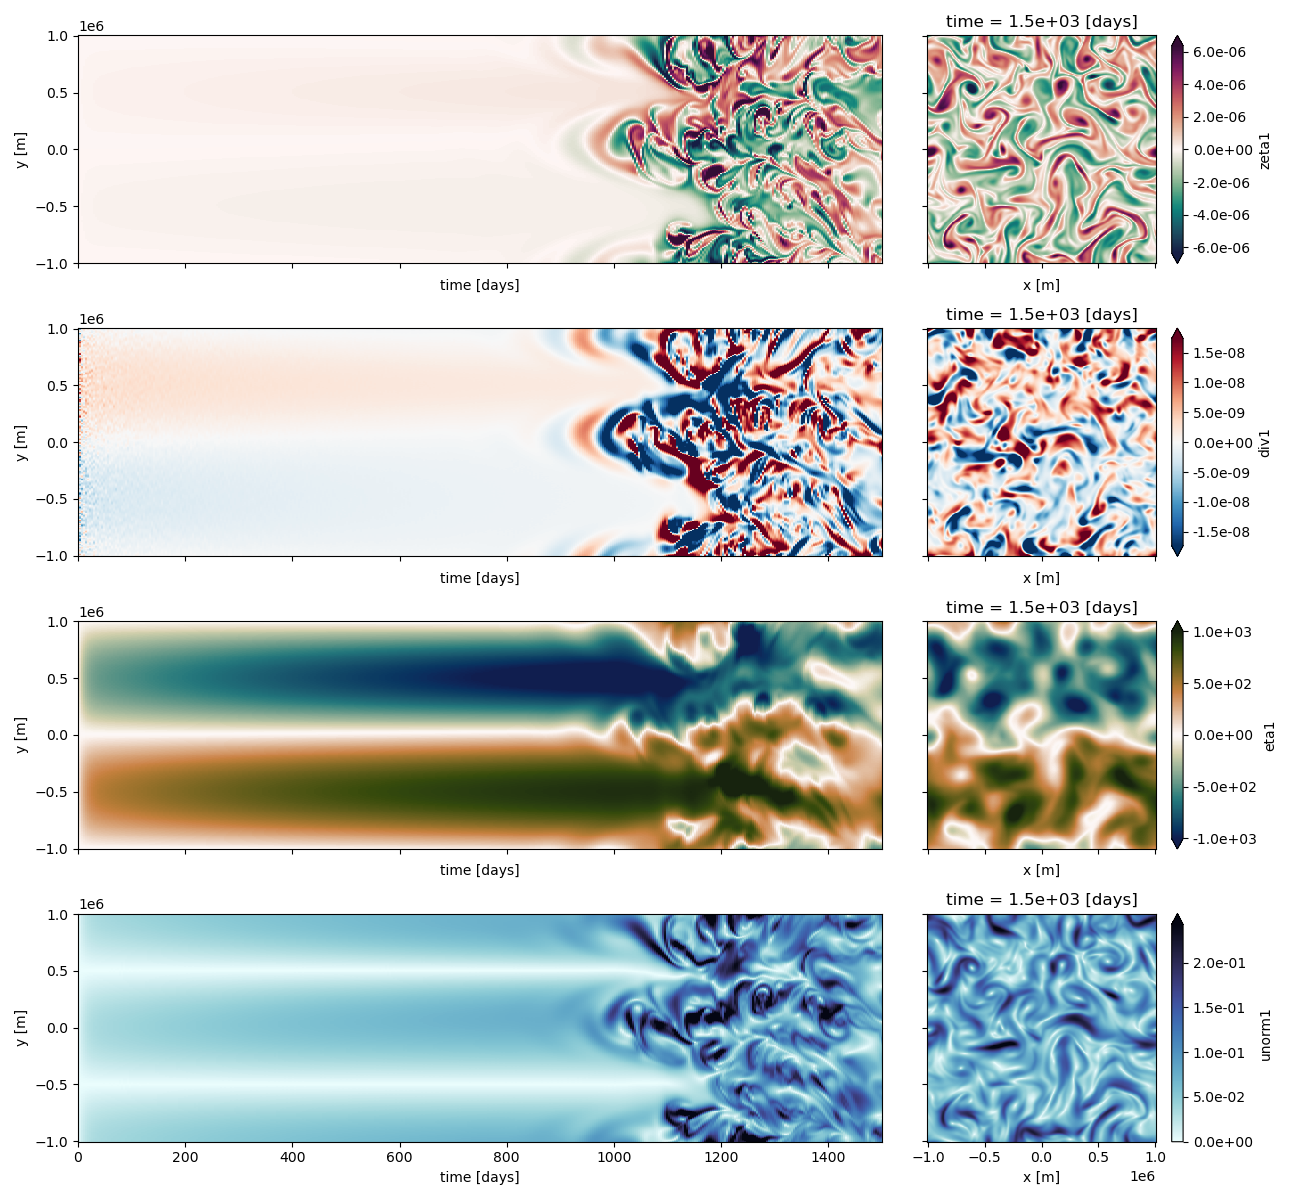
\includegraphics[width=0.5\textwidth]{figures/tests/2023-06-15_hovmoller1_t=1500days_fft.png} & 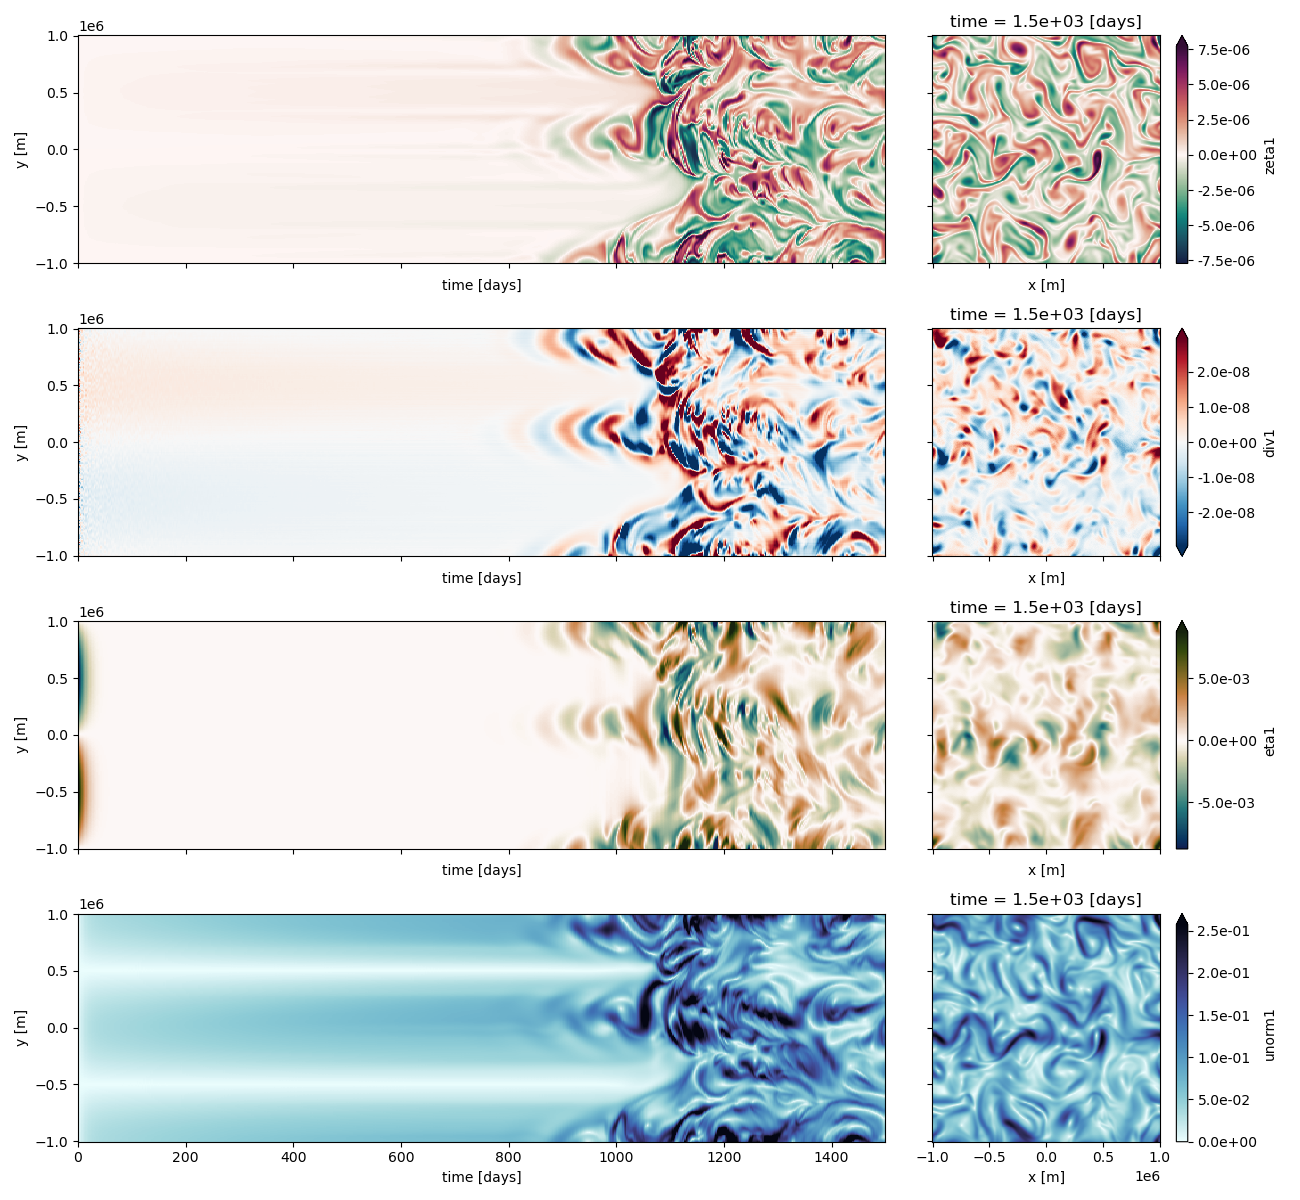
\includegraphics[width=0.5\textwidth]{figures/tests/2023-06-19_hovmoller1_t=1500days_mud.png}\\[0pt]
\end{tabular}
\end{table}

\newpage
\section{{\bfseries\sffamily DONE} Comparatif : nombre de cycles Multigrid}
\label{sec:org9973f4e}
Dans la sous-routine \emph{MUDPACK} que nous utilisons, un des paramètre est dénommé \emph{maxcy}.
Concrétement, ce nombre entier décrit le nombre maximum de cycles \emph{multigrid} entre la plus grande et petite échelle.
Comme la sous-routine est assez demandante en temps de calcul, j'ai testé de mettre seulement un seul cycle.
Essentiellement, on ne voit aucune différence.

\begin{table}[htbp]
\caption{\label{tab:org0ffa5bd}Diagrammes de Hovmoller entre 0 et 100 jours. À gauche, MUDPACK à 5 cycles complets. À droite, 1 seul cycle.}
\centering
\begin{tabular}{ll}
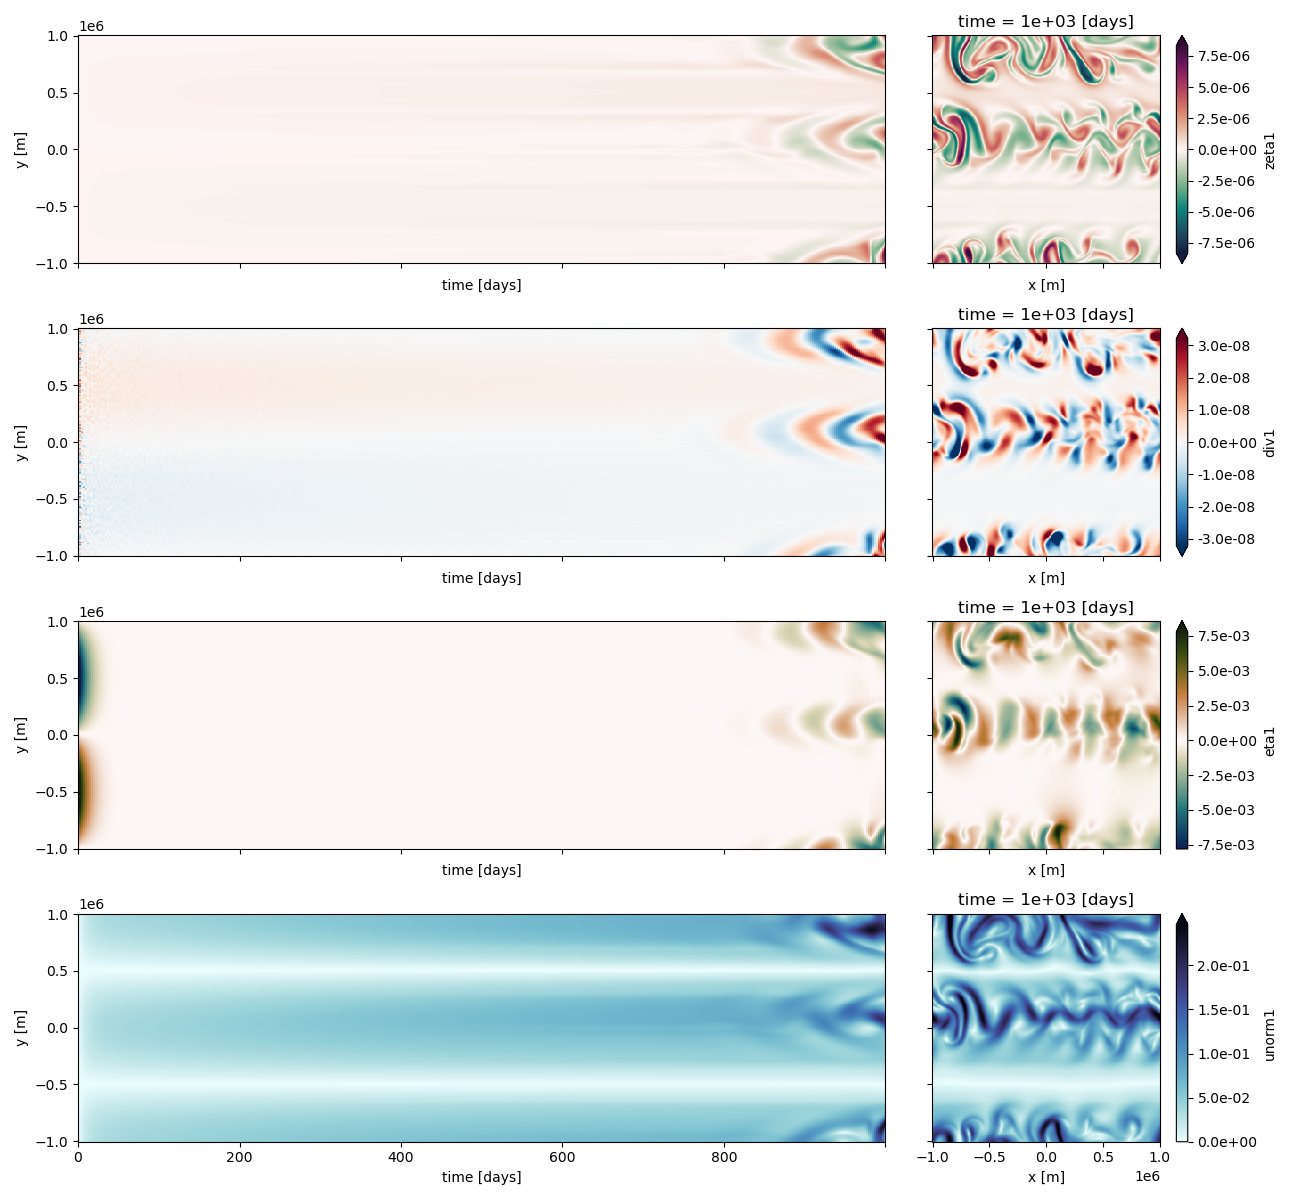
\includegraphics[width=0.5\textwidth]{figures/tests/2023-06-19_hovmoller1_t=1000days_mud.png} & 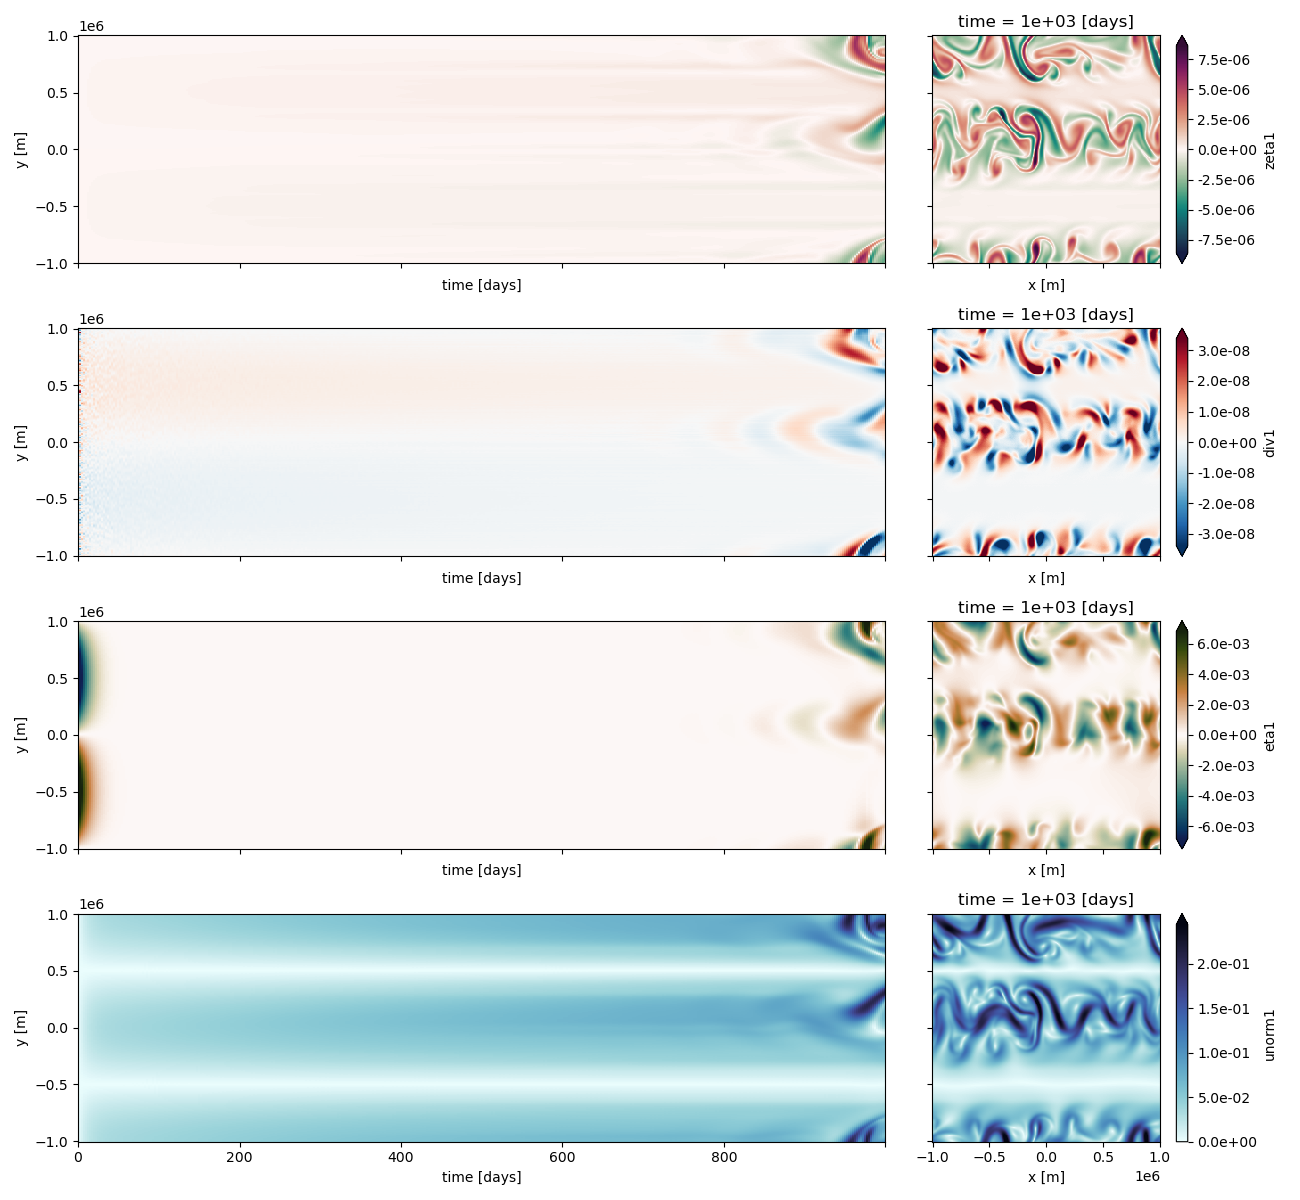
\includegraphics[width=0.5\textwidth]{figures/tests/2023-06-19_hovmoller1_t=1000days_mud_maxcy1.png}\\[0pt]
\end{tabular}
\end{table}
\end{document}